\section{Ecore Metamodell}
Im Originalpaper \cite{gerhart2015approach} wird an vielen Stellen ein Bezug zu Ecore hergestellt, besonders in Abschnitt \ref{sec:evaluation}. Damit diese Bezüge und Vergleiche zwischen MoDiGen und Ecore anschaulicher werden wird in diesem Abschnitt ein Überblick über Ecore eingeschoben. Es beinhaltet einen Ausschnitt aus der Architektur des ECore-Modells, der im Zusammenhang mit dem Originalpaper besonders relevant ist.

%In diesem Absatz wird der relevante Ausschnitt aus der Architektur des ECore-Modells n\"aher beschrieben, da es im Abschnitt \ref{sec:evaluation} zum Vergleich herangezogen wird.

\subsection{Architektur}
Der zugrundeliegende Aufbau des ECore-Modells bildet weitaus mehr modellierungs Möglichkeiten ab, als der Aufbau von MoDiGen (siehe dazu \cite{eclipse_ecore}). Dazu gehören u.a. Pakete (EPackage), Operationen mit Parametern (EOperation, EParameter) und EFactory durch die sich Instanzerzeugung oder Konvertierungen modellieren lassen. Diese Bestandteile des ECore-Modells werden bei der folgenden Betrachtung ausgelassen, da sie keinen Beitrag zum Verständnis der Evaluierung in Abschnitt \ref{sec:evaluation} leisten.\\
\\
Eine Klasse \texttt{EClass} hat einen Namen und besitzt Attribute \texttt{EAttribute} und Referenzen \texttt{EReference}. Die Referenz ist über eine Komposition modelliert und kann nicht ohne eine zugeordnete Klasse existieren. Eine abstrakte Klasse \texttt{ETypedElement} die von \texttt{EStructuralFeature} geerbt wird enth\"alt Attribute wie \textit{upper-} und \textit{lowerBound}, durch die sich Multiplizitäten festlegen lassen. Neben \texttt{EReference} erbt auch \texttt{EAttribute} von \texttt{EStructuralFeature}. Der Datentyp eines Attributes wird durch eine Assoziation zu \texttt{EDataType} festgelegt. Ecore definiert dabei 21 Java Datentypen, wie u.a. \texttt{EBoolean}, \texttt{EByte} und \texttt{EChar} sowie 10 zus\"atzliche (u.a. \texttt{EDate} und \texttt{EEList}). Das Modell ist unter \cite{eclipse_ecore} vollst\"andig einzusehen.

\begin{figure}
\centering
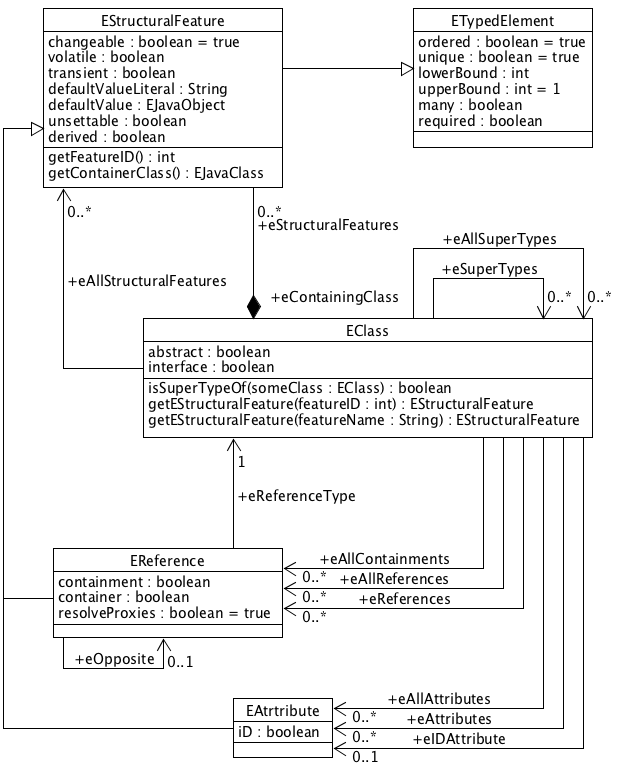
\includegraphics[width=\linewidth]{Abschnitte/Abbildungen/Grafiken/EMF}
\caption{Auschnitt aus dem Ecore-Metamodell des Eclipse Modelling Frameworks \cite{eclipse_ecore}}
\label{fig:emf-ecore-kd}
\end{figure}


Das Listing \ref{lst:ecore-modell} zeigt wie die Klasse \texttt{Female} aus Abbildung \ref{fig:Family-Tree-Model} als ECore-Modell in XML abgespeichert wird. Die Referenzen \textit{isWife} und \textit{isMother} werden durch \texttt{eStructuralFeatures} mit dem XML-Typ \textit{ecore:EReference} als Kindelemente beschrieben. Die entsprechenden Attribute wie \textit{eType} und \textit{upperBound} sind als XML-Attribute von \texttt{eStructuralFeatures} vermerkt.

\begin{lstlisting}[caption=Auszug der Klasse Female aus Abbildung \ref{fig:Family-Tree-Model} als ECore in XML, label=lst:ecore-modell, language=xml, basicstyle=\small, tabsize=4,frame=single, showstringspaces=false, numbers=left, keywordstyle=\bfseries, breaklines=true]
[...]
  <eClassifiers xsi:type="ecore:EClass" name="Female" eSuperTypes="#//Person">
    <eStructuralFeatures xsi:type="ecore:EReference" name="isWife" eType="#//Male"/>
    <eStructuralFeatures xsi:type="ecore:EReference" name="isMother" upperBound="-1" eType="#//Person"/>
  </eClassifiers>
[...]
\end{lstlisting}
